\chapter{Teor\'ia de Errores}

\section{Introducci\'on}

Esta secci\'on se centrar\'a en la teor\'ia de errores en el contexto de las mediciones experimentales. Se explorar\'an los tipos de errores, incluyendo errores sistem\'aticos y aleatorios, y se discutir\'an estrategias para minimizar y cuantificar estos errores. Adem\'as, se introducir\'an m\'etodos para calcular incertidumbres.

Cuando se realiza la medida de una magnitud f\'isica un cierto numero de veces, se observa que no todos los valores son iguales entre si y l\'ogicamente nos preguntamos �Cu\'al es el valor correcto? �Por qu\'e los valores obtenidos son diferentes?

Antes de contestar estas preguntas, debemos decir que ninguna medici\'on  puede dar un valor absolutamente exacto de una cantidad f\'isica. Es por ello que, cuando hablamos del valor ``verdadero'' de una magnitud f\'isica o valor exacto (valor que tendr\'ia la magnitud si no estuviese afectada de ning\'un tipo de error) debemos entenderlo como una abstracci\'on.

Se puede emplear los m\'etodos e instrumentos t\'ecnicos m\'as perfeccionados y de todos modos ninguna medici\'on lleva a un valor exacto, sino a la posibilidad de indicar un intervalo en el cual debe estar comprendido el ``verdadero valor'' para la magnitud medida.

Por ejemplo, si se mide la longitud de un objeto con una regla graduada, se puede decir que el resultado tiene una incertidumbre de $\pm 1$ mm, y  el resultado se puede escribir como  $5,5 \pm 0,1$ cm. Pero si se utiliza un vernier, el cual permite obtener una medida con m\'as precisi\'on, el resultado ser\'ia $5,530 \pm 0,005$ cm.

\section{Exactitud, precisi\'on y sensibilidad}

\begin{itemize}
\item Exactitud: se refiere al grado de concordancia entre el valor �verdadero�\footnote{Por ahora lo que entendemos como valores �verdaderos� luego los definiremos como valores medios.}  y el medido experimentalmente. Decimos que un aparato es exacto si las medidas realizadas con \'el son todas muy pr\'oximas al valor �verdadero�de la magnitud medida.
\item Precisi\'on: tiene que ver con la concordancia entre las medidas de una misma magnitud realizadas en condiciones sensiblemente iguales, un aparato es m\'as preciso cuando la diferencia entre diferentes mediciones de una misma magnitud sean muy peque\~nas. Notemos que la exactitud normalmente implica precisi\'on, pero la afirmaci\'on inversa no es cierta, ya que pueden existir aparatos muy precisos que posean poca exactitud, debido a errores sistem\'aticos, como por ejemplo el �error del cero�. 

Por lo tanto, precisi\'on y exactitud no son sin\'onimos, la precisi\'on tiene que ver con la capacidad que tiene el instrumento para tomar una medida mientras que exactitud tiene que ver con el hecho de lo cerca que pueda estar una medici\'on al valor real.

\item Sensibilidad: se relaciona con el valor m\'inimo de la magnitud que es capaz de medir un aparato. Cuando decimos que la sensibilidad de una balanza es de 1 mg, significa que para masas inferiores a este valor la balanza no muestra ninguna desviaci\'on. Por lo general consideramos la sensibilidad de un aparato de medida como el valor de la divisi\'on m\'as peque\~na de la escala de medida. 

As\'i como es importante no confundir precisi\'on con exactitud, tambi\'en es importante no confundir precisi\'on y sensibilidad.
\end{itemize}

\section{Tipos de errores en las mediciones}

\subsection{Errores sistem\'aticos}
Son aquellos errores que afectan los resultados en una misma direcci\'on y pueden ser causados por:
\begin{enumerate}
\item Defectos y errores de calibraci\'on de los instrumentos. Por ejemplo, si el cero del tambor de un tornillo microm\'etrico no coincide con el cero de la escala fija, se introducir\'a una desviaci\'on que ser\'a igual para todas las medidas realizadas. Esto se puede remediar recalibrando el instrumento.
\item El observador (errores personales). Puede introducir errores por efectos de paralaje. Se deben evitar estando consciente de las causas que los originan.
\item Variaci\'on de las condiciones ambientales. En este caso el observador no tiene control.
\item El m\'etodo empleado.  En este caso, los errores solo se hacen evidentes, si se cambia el m\'etodo.
\end{enumerate}
Para tratar estos errores de manera segura es necesario poder controlar el correcto funcionamiento de los equipos de medida.

\subsection{Errores casuales o accidentales}

Son aquellos errores producto de una contribuci\'on de fuentes incontrolables que van desplazando aleatoriamente el valor medido por encima y por debajo de su valor real, esto hace que las medidas den resultados diferentes. Se les conoce tambi\'en como errores aleatorios o estad\'isticos.  Los errores casuales, a diferencia de los errores sistem\'aticos, son inevitables y est\'an presentes en todo experimento porque son una consecuencia de  m\'ultiples fluctuaciones incontrolables e independientes de los factores que intervienen en la realizaci\'on de una medici\'on.

Pueden ser causados por:
\begin{enumerate}
\item Condiciones ambientales fluctuantes, tales como: temperatura, presi\'on variaciones de voltaje en la linea.
\item Oscilaciones de los mecanismos propios del instrumento de medida.
\item El observador.
\item Factores que puedan introducir errores que contribuyen al error total en los que podemos mencionar los siguiente: vibraciones mec\'anicas, se\~nales par\'asitas en instrumentos electr\'onicos, defectos de f\'abrica, etc.
\end{enumerate}

Como se trata de errores al azar, es casi imposible decidir si el promedio de las medidas se aleja hacia arriba o hacia abajo del valor exacto, por esto dicho error se expresa acompa\~nado del signo de indeterminaci\'on $\pm$ . En el caso de errores sistem\'aticos se puede al menos en principio, determinar su signo.

\subsection{Errores de precisi\'on}

Los equipos de medici\'on poseen escalas o d\'igitos y la divisi\'on m\'as peque\~na de la escala o el \'ultimo d\'igito determina la m\'inima diferencia de magnitud que puede apreciar el equipo, es decir: su resoluci\'on.

Una cinta m\'etrica se encuentra dividida en cent\'imetros y mil\'imetros, por lo tanto, las medidas que se realicen con la cinta nos permitir\'a conocer la longitud de un objeto con un error aproximado de 1 mm. En el caso de que queramos disminuir el error de la medida debemos utilizar un dispositivo de medici\'on que tenga una mayor resoluci\'on.

Este tipo de error se le conoce como el error de precisi\'on y se debe a la resoluci\'on, sensibilidad, del aparato de medida. Suele designarse con $\varepsilon_p$

\section{La escritura de los resultados de una medici\'on}

Al medir una magnitud $x$ y conocer el error involucrado en la medici\'on $\Delta x$ debemos expresar la medida de la siguiente manera
\begin{equation}
x=x_0 \pm \Delta x \quad \text { [unidades] }
\end{equation}
\begin{itemize}
\item $x_0$ es el valor de la medida
\item  $\Delta x$ es la incertidumbre o el error de la medida
\end{itemize}
Nota: la medida y el error se deben dar en las mismas unidades.

Por ejemplo, con una cinta m\'etrica se ha medido la altura de una persona. El resultado obtenido es de $1.68 \mathrm{~m}$, y el error cometido es $1 \mathrm{~cm}$. La forma correcta de expresar el resultado de la medida es:
$$
\text { altura }=1,68 \pm 0,01 \mathrm{~m}\,.
$$

\subsection{Error absoluto y error relativo}

Cuando medimos una magnitud f\'isica cuyo valor ``verdadero'' es $x_0$, lo que obtenemos por el proceso de medici\'on es un  valor  $x$ de la medida, el {\bf error absoluto} de dicha medida es la siguiente diferencia
\begin{equation}
\Delta {x}=|{x}-{x}_0| \,,
\end{equation}
en donde suponemos que $\Delta x \ll\left|x_0\right|$.

El error absoluto nos da una medida de la desviaci\'on, en t\'erminos absolutos, respecto al valor ``verdadero". 

Conocido el el error absoluto podemos calcular el {\bf error relativo} de dicha medida: 
\begin{equation}
\varepsilon=\frac{\Delta x}{x_0},
\end{equation}
de manera que en forma porcentual se puede expresar como $\varepsilon \times 100 \%$.

Cuando vayamos a escribir el resultado de una medici\'on para una magnitud M de debe indicar el grado de incertidumbre de la manera siguiente
\begin{equation}
\mathrm{M}=x \pm \Delta x \quad \text { [unidades] } \,.
\end{equation}

Es muy com\'un escribir el error absoluto con solo una cifra significativa, al menos que se indique lo contrario. Si el error se ha obtenido con m\'as de una cifra, se deber\'a a proceder a suprimir las posteriores por el m\'etodo del redondeo.  El valor de la magnitud debe tener s\'olo las cifras necesarias para que su \'ultima cifra significativa sea del mismo orden decimal que la \'ultima del error absoluto, tambi\'en llamada cifra de acotamiento.

Escribir el error con una o dos cifras significativas es una decisi\'on un poco arbitraria, y depender\'a del error introducido. Por ejemplo, si tenemos un error de 0,89 m y lo redondeamos a 0,9, la diferencia introducida es ligeramente superior al 1 \%, valor que podr\'ia justificar el redondeo y expresar el error de una manera m\'as sencilla; pero si un error de 1,4 m lo redondeamos a 1 m, la diferencia es cercana a un 40 \%, algo dif\'icilmente justificable. 

En la siguiente tabla mostramos algunos ejemplos de medidas redondeando a una cifra significativa el error absoluto
$$
\begin{array}{|c|c|}
\hline \text { Incorrecto } & \text { Correcto } \\ \hline
\hline 3,319 \pm 0,123 & 3,3 \pm 0,1 \\
\hline 6,5 \pm 0,09 & 6,50 \pm 0,09 \\
\hline 428,364 \pm 0,28 & 428,4 \pm 0,3 \\
\hline 0,01695 \pm 0,0056 & 0,017 \pm 0,006 \\
\hline 46276 \pm 1563 & (46 \pm 2) \times10^3 \\
\hline
\end{array}
$$


\section{Mediciones directas}

Cuando hacemos una medida directamente de un aparato de medici\'on decimos que hacemos una medida directa. En lo que sigue vamos a estudiar el tratamiento de los errores suponiendo  que las medidas est\'an libres de errores sistem\'aticos. 

\subsection{C\'alculo de los errores con una sola medida}

En el caso de realizar una sola medida $x$ de una magnitud, el error cometido vendr\'a  dado \'unicamente por el error de precisi\'on del aparato utilizado, es decir,  $ \varepsilon_p= \Delta x$ . 

Pero es necesario diferenciar si la medida la hacemos con un aparato anal\'ogico o digital.

\begin{itemize}
\item Anal\'ogico: el error de precisi\'on se toma como la mitad de la divisi\'on mas peque\~na  que puede medir el instrumento, es decir, la mitad de su sensibilidad.
\begin{equation}
\varepsilon_p= \frac{\text{divisi\'on m\'as peque\~na}}{2} 
\end{equation}

Por ejemplo, supongamos que un amper\'imetro anal\'ogico tiene una escala de lectura que aprecia valores hasta d\'ecimas de amperio (sensibilidad: S=0,1 A) y, al hacer una medida, la aguja se queda entre 0,6 A y 0,7 A. En ese caso, se podr\'a tomar como valor experimental de la corriente $I = 0,65$ A y como error absoluto $\varepsilon_p=(0,1)/2 = 0,05$ A. Se dir\'a que la intensidad de corriente es de $0,65 \pm 0,05$ A.

Para una regla  dividida mil\'imetros el error de precisi\'on en mil\'imetros es
de $ \varepsilon_p$ = 0,5 mm.

\item Digital: el error de precisi\'on es la m\'inima magnitud que puede medir el instrumento.
\begin{equation}
 \varepsilon_p = \text{m\'inima magnitud medible}
\end{equation}

Por ejemplo, supongamos que un cron\'ometro digital que mide hasta mil\'esimas de segundo (sensibilidad: S = 1 ms) nos permite medir el per\'iodo de oscilaci\'on de un p\'endulo en $T = 882$ ms. El error absoluto en este caso es $\varepsilon_p=1$ ms. Por lo tanto, el resultado se debe escribir como: $T=882 \pm 1$ ms.

\end{itemize}

\subsection{C\'alculo de los errores en una serie de medidas}

En esta secci\'on nos referimos solo a los errores casuales, cuyo c\'alculo necesita del uso de la teor\'ia estad\'istica. Esta teor\'ia es v\'alida cuando el n\'umero de medidas que ser realiza es grande.

En el laboratorio elemental se considera que el n\'umero de medidas es grande, cuando $n \geq 25$. Pero no debe considerarse a este n\'umero como un valor fijo. Para otros autores, la separaci\'on entre un n\'umero grande y uno peque\~no de medidas  puede variar.

Hemos dicho que cuando se realiza una serie de medidas de una magnitud lo m\'as probable es que ellas sean diferentes, entonces uno se pregunta �cu\'al es la mejor medida?

\subsubsection{C\'alculo de errores en un n\'umero peque\~no de medidas}

Para contestar estas preguntas se acostumbra utilizar algunas definiciones necesarias. 

\paragraph{Valor medio aritm\'etico:} se define como el cociente entre la suma de las medidas: $x_1, x_2, \ldots, x_N$ y el n\'umero de $N$ medidas realizadas.
\begin{equation}
\bar{x}=\frac{x_1+x_2+x_3+\ldots+x_N}{N}=\frac{1}{N} \sum_{i=1}^N x_i
\end{equation}

Es decir, la media de las medidas es el valor m\'as probable de la magnitud. Se puede mostrar que $\bar{x}$ es el valor m\'as cercano al valor verdadero (desconocido) de una medida.

\paragraph{Error absoluto de una medida:} como mencionamos con anterioridad, se corresponde al valor absoluto de la diferencia del valor medio respecto a cada medida.
\begin{equation}
\Delta x_i=\left|\bar{x}-x_i\right|
\label{errabs}
\end{equation}

\paragraph{Error medio absoluto de una serie de medidas:} se define como el valor medio aritm\'etico de los errores absolutos de cada medida.
\begin{equation}
\overline{\Delta x}=\frac{\Delta x_1+\Delta x_2+\Delta x_3+\ldots+\Delta x_N}{N}=\frac{1}{N} \sum_{i=1}^N \Delta x_i \,.
\label{errmedabs}
\end{equation}

\paragraph{Error relativo de una serie de medidas:} es dado por el cociente entre el error medio absoluto y el valor medio aritm\'etico de las medidas.
\begin{equation}
\varepsilon_x=\frac{\overline{\Delta x}}{\bar{x}} \,.
\label{errel}
\end{equation}

\paragraph{Error porcentual:} se define como el producto del error relativo por 100
\begin{equation}
\varepsilon_{\%}=\varepsilon_x \times 100 \,.
\label{errpor}
\end{equation}

\paragraph{Dispersi\'on $D$:} la diferencia entre los valores extremos de las medidas:
\begin{equation}
D=x_{\text {max}}-x_{\text {min}} \,.
\label{disper}
\end{equation}

\paragraph{Dispersi\'on porcentual $D_{\%}$:} definido por
\begin{equation}
D_{\%}= \frac{D}{\bar{x}} \cdot 100  
\label{disperpor}
\end{equation}



\paragraph{Ejemplo 1.} Para ilustrar lo descrito antes, realizaremos el siguiente ejercicio:

Se quiere determinar el volumen de un cilindro y por lo tanto es necesario medir la altura y el di\'ametro del mismo. La medida de la altura se hizo una vez con una cinta m\'etrica, mientras que la del di\'ametro se realiz\'o cinco veces con un vernier de apreciaci\'on $0,005 \mathrm{~cm}$.
$$
\text { altura }=h=(10,2 \pm 0,1) \mathrm{cm}
$$

$$
\begin{array}{|l|l|l|l|l|l|}
\hline d=\text { di\'ametro }(\mathrm{cm}) & 1,780 & 1,780 & 1,780 & 1,790 & 1,790 \\
\hline
\end{array}
$$

El di\'ametro promedio es:
$$
\bar{d}=\frac{1,780+1,780+1,780+1,790+1,790}{5}=1,784 \mathrm{~cm}
$$
En este caso la dispersi\'on es:
$$
D=1,790-1,780 = 0,01 \,\Rightarrow \, D_{\%}= \frac{0,01}{1,784} \cdot 100  = 0,6 \%
$$

Los errores absolutos para cada medida del di\'ametro son los siguientes:
$$
\begin{aligned}
& \Delta d_1=|1,784-1,780|=0,004 \mathrm{~cm} \\
& \Delta d_2=|1,784-1,780|=0,004 \mathrm{~cm} \\
& \Delta d_3=|1,784-1,780|=0,004 \mathrm{~cm} \\
& \Delta d_4=|1,784-1,790|=0,006 \mathrm{~cm} \\
& \Delta d_5=|1,784-1,790|=0,006 \mathrm{~cm}
\end{aligned}
$$
El error absoluto del di\'ametro:
$$
\overline{\Delta d}=\frac{0,004 \mathrm{~cm}+0,004 \mathrm{~cm}+0,004 \mathrm{~cm}+0,006 \mathrm{~cm}+0,006 \mathrm{~cm}}{5}=0,005 \mathrm{~cm}
$$
El error relativo del di\'ametro:
$$
\varepsilon_d=\frac{\overline{\Delta d}}{\bar{d}}=\frac{0,005 \mathrm{~cm}}{1,784 \mathrm{~cm}}=0,0028 .
$$
El error porcentual para el di\'ametro:
$$
\varepsilon_{\%}=\varepsilon_d \times 100=0,0028 \times 100=0,28 \%
$$
El error relativo para la altura:
$$
\varepsilon_h=\frac{\Delta h}{h}=\frac{0,1 \mathrm{~cm}}{10,2 \mathrm{~cm}}=0,01 .
$$
El error porcentual para la altura:
$$
\varepsilon_{\%}=\varepsilon_h \times 100=0,01 \times 100=1 \% .
$$

Por lo tanto:
$$
h=(10,2 \pm 0,1) \mathrm{~cm} \quad y \quad d= (1,784 \pm 0,005)\mathrm{~cm}
$$

Vamos a reproducir el ejemplo anterior en Python. Primero que todo debemos incorprar las librerias {\bf numpy} y {\bf matplotlib}

\begin{lstlisting}[language=Python]
from numpy import *
import matplotlib.pyplot as plt
\end{lstlisting}
   
Luego introducimos los datos como un arreglo
\begin{lstlisting}[language=Python]    
d = array([1.780, 1.780, 1.780, 1.790, 1.790])
print('Num de datos:',         len(d)  )
print('promedio:',             mean(d), 'cm' )
print('suma:',                 sum(d)  )
\end{lstlisting}
\begin{tcolorbox}[width=\textwidth,colback={ghostwhite}]    
{\small Num de datos: 5 \\
promedio: 1.784 cm\\
suma: 8.92
}
\end{tcolorbox} 

Podemos calcular la dispersi\'on de la siguiente manera
\begin{lstlisting}[language=Python]    
# Valores m\'aximo y m\'inimos del conjunto de datos
print('valor m\'aximo:',  amax(d))
print('valor m\'inimo:',  amin(d))
print('dispersi\'on:',   (amax(d)-amin(d)).round(2))
print('dispersi\'on porcentual:', ((amax(d)-amin(d))/mean(d)*100).round(1),'%')
\end{lstlisting}
\begin{tcolorbox}[width=\textwidth,colback={ghostwhite}]   
{\small valor m\'aximo: 1.79 \\
valor m\'inimo: 1.78 \\
dispersi\'on: 0.01\\
dispersi\'on porcentual: 0.6 $\%$
}
\end{tcolorbox} 

Para el error absoluto del di\'ametro
\begin{lstlisting}[language=Python]    
Delta_d=(sum(abs(mean(d)-d))/len(d)).round(3)
Delta_d
\end{lstlisting}
\begin{tcolorbox}[width=\textwidth,colback={ghostwhite}] 
{\small 
0.005
}
\end{tcolorbox} 

Para el error relativo del di\'ametro
\begin{lstlisting}[language=Python]    
err_d=(Delta_d/mean(d)) # error relativo 
err_dp=(e_d*100)    # error porcentual

print('error relativo:', err_d.round(4))
print('error porcentual:', err_dp.round(2),'%')
\end{lstlisting}
\begin{tcolorbox}[width=\textwidth,colback={ghostwhite}]  
{\small error relativo: 0.0028 \\
error porcentual: 0.28 \%
}
\end{tcolorbox} 

\subsubsection{C\'alculo de errores en un n\'umero grande de medidas}

Supongamos que, un estudiante necesita conocer el di\'ametro de un tubo de vidrio, para lo cual realiza  25 medidas, Tabla \ref{diametros}. El instrumento utilizado fue un tornillo microm\'etrico de apreciaci\'on $0,01 \mathrm{~mm}$.
\begin{table}[h]
\begin{center}
\begin{tabular}{|c|c|c|c|c|c|}
\hline$N^{\circ}$ de la medida & $\mathrm{d}(\mathrm{mm})$ & $N^{\circ}$ de la medida & $\mathrm{d}(\mathrm{mm})$ & $N^{\circ}$ de la medida & $\mathrm{d}(\mathrm{mm})$ \\
\hline \hline 1 & 15,12 & 10 & 15,14 & 19 & 15,14 \\
\hline 2 & 15,10 & 11 & 15,15 & 20 & 15,13 \\
\hline 3 & 15,15 & 12 & 15,14 & 21 & 15,15 \\
\hline 4 & 15,17 & 13 & 15,13 & 22 & 15,13 \\
\hline 5 & 15,14 & 14 & 15,14 & 23 & 15,11 \\
\hline 6 & 15,16 & 15 & 15,13 & 24 & 15,13 \\
\hline 7 & 15,14 & 16 & 15,13 & 25 & 15,15 \\
\hline 8 & 15,12 & 17 & 15,14 & & \\
\hline 9 & 15,12 & 18 & 15,14 & & \\
\hline
\end{tabular}
\end{center}
\caption{Medidas del di\'ametro $d$ de un tubo}
\label{diametros}
\end{table}

�C\'omo presentar estas medidas gr\'aficamente? Una manera es por me�dio de un histograma, el cual no es m\'as que un gr\'afico del n\'umero de veces que ocurre una medida (frecuencia) como funci\'on del valor de \'esta.

El histograma se construye de la forma siguiente: Se divide el conjunto de valores medidos en intervalos iguales y se cuenta el n\'umero de veces que ocurre el valor de la medici\'on en cada intervalo. El ancho de cada intervalo es arbitrario y generalmente se escoge el m\'as conveniente. 

Con los valores de la tabla anterior \ref{diametros} y escogiendo como el ancho del intervalo en  0,01 mm, las frecuencias de las medidas se muestran en la tabla \ref{histo1}. 

\begin{table}[h]
\begin{center}
\begin{tabular}{|c|c|}
\hline Intervalo $(\mathrm{mm})$ & Frecuencia \\
\hline \hline \hline $15,095-15,105$ & 1 \\
\hline $15,105-15,115$ & 1 \\
\hline $15,115-15,125$ & 3 \\
\hline $15,125-15,135$ & 6 \\
\hline $15,135-15,145$ & 8 \\
\hline $15,145-15,155$ & 4 \\
\hline $15,155-15,165$ & 1 \\
\hline $15,165-15,175$ & 1 \\
\hline
\end{tabular}
\end{center}
\caption{Frecuencias de las medidas de la tabla \ref{diametros}}
\label{histo1}
\end{table}

Para hacer un histograma podemos volver al Pyhton
\begin{lstlisting}[language=Python]    
d = array([15.12, 15.10, 15.15, 15.17, 15.14, 15.16, 15.14, 15.12, 
           15.12, 15.14, 15.15, 15.14, 15.13, 15.14, 15.13, 15.13, 
           15.14, 15.14, 15.14, 15.13, 15.15, 15.13, 15.11, 15.13, 
           15.15])
plt.hist(d,edgecolor = "white", bins=8)
plt.xlabel('Di\'ametros')
plt.ylabel('Frecuencia')
plt.title("histograma")
plt.show()
\end{lstlisting}
\begin{figure}[h]
\begin{center}
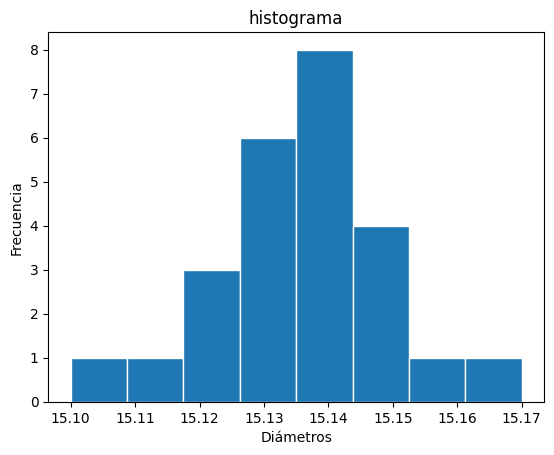
\includegraphics[height=2.5in,width=3.6in]{figuras/fig03}  
\caption{Histograma para los datos de la tabla \ref{diametros}.}
\label{gauss2}
\end{center}
\end{figure}

Si se efectuaran otras 25 mediciones, el histograma respectivo ser\'ia probablemen�te diferente al mostrado en \ref{gauss2}, y si se continuase haciendo medidas del di\'ametro hasta un n\'umero $n$ muy grande y se realizara un nuevo histograma de ellas, tomando los intervalos m\'as peque\~nos, se obtendr\'ia una curva continua, llamada gaussiana o curva de Gauss, ver gr\'afica \ref{gauss3}. De la curva de Gauss podemos extraer la informaci\'on, que nos permite decidir que tan confiables son los valores obtenidos en las medidas realizadas. 
\begin{figure}[h]
\begin{center}
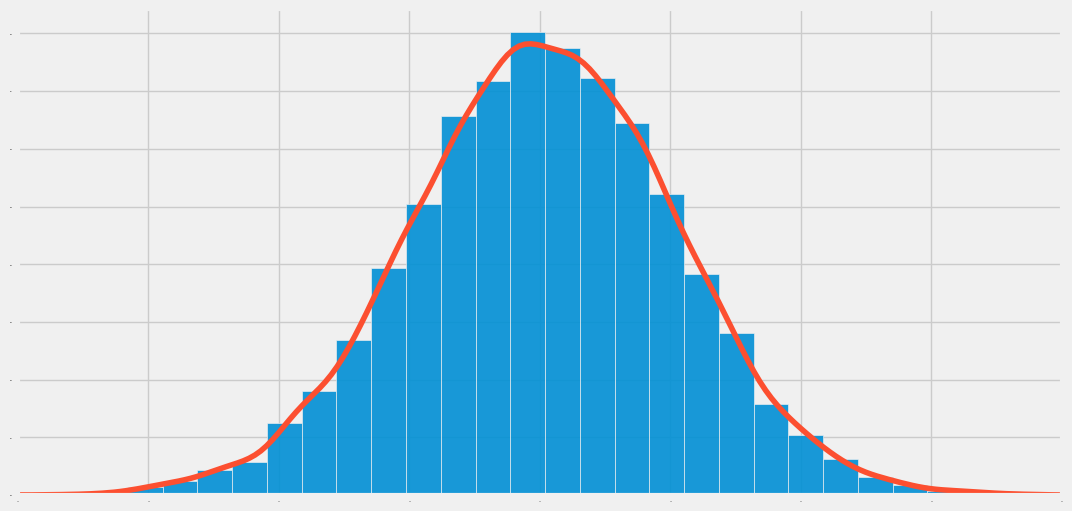
\includegraphics[height=2.5in,width=3.6in]{figuras/fig04}  
\caption{Curva de Gauss para un n\'umero $n$ muy grande de medidas.}
\label{gauss3}
\end{center}
\end{figure}

Adem\'as del valor medio aritm\'etico $\bar{x}$ tambi\'en podemos definir:
\paragraph{Desviaci\'on de cada medida respecto al valor medio:} 
corresponde a la diferencia entre el valor medio y cada medida y se denota por $\Delta x_i$.
\begin{equation}
\Delta x_i=\bar{x}-x_i
\end{equation}
Las desviaciones pueden ser positivas o negativas, lo cual nos se\~nala que las medidas caen a uno u otro lado del valor medio.

\paragraph{Desviaci\'on est\'andar:} Se define como:
\begin{equation}
\sigma=\sqrt{\frac{\sum_{i=1}^N\left(\bar{x}-x_i\right)^2}{(N-1)}}
\label{des1}
\end{equation}
cuando el n\'umero de medidas no es lo suficientemente grande.

En el caso que se tengan varios conjuntos de medidas ($N$ grande), la desviaci\'on est\'andar est\'a dada por:
\begin{equation}
\sigma=\sqrt{\frac{\sum_{i=1}^N\left(\bar{x}-x_i\right)^2}{N(N-1)}}
\end{equation}

La curva de Gauss dibujada en la figura \ref{gauss2}, ayuda a visualizar las definiciones dadas para el valor medio y la desviaci\'on est\'andar.
\begin{figure}[h]
\begin{center}
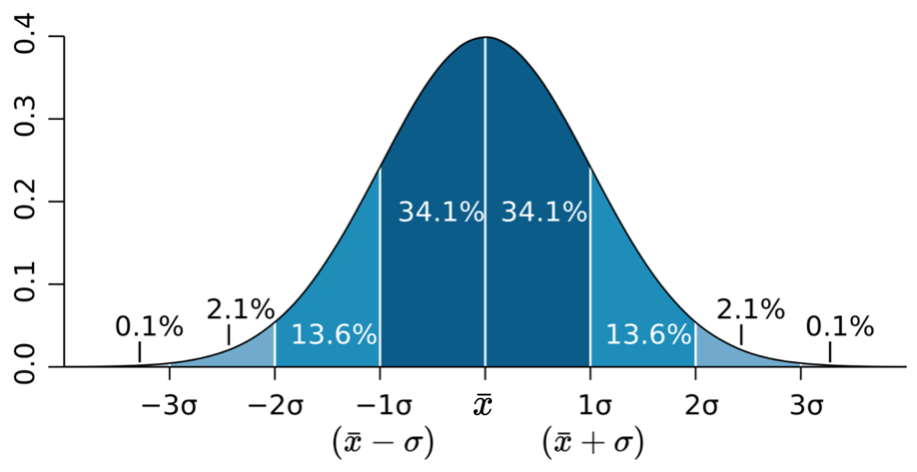
\includegraphics[height=2.1in,width=3.6in]{figuras/fig05}  
\caption{Curva de distribuci\'on de Gauss mostrando la posici\'on de $\bar{x}$ y $\sigma$}
\label{gauss4}
\end{center}
\end{figure}

Podemos notar que los valores de las mediciones tienden a agruparse alrededor de un punto central: la media. La representaci\'on de los datos es sim\'etrica a ambos lados de la media y las desviaciones est\'andares quedan situadas a igual distancia unas de otras. 

Notemos tambi\'en que la proporci\'on de las medidas  situada entre la media y las desviaciones es una constante, por ejemplo: $\bar{x} \pm 1 \sigma$ cubre el 68,3 \% de las mediciones. Mientras que $\bar{x} \pm 3 \sigma$ cubre el 99,7 \%. 

\paragraph{Error probable $\left(\varepsilon_p\right)$}

Se define como la desviaci\'on respecto al valor medio, que divide la mitad derecha (o izquierda) del \'area bajo la curva de Gauss en dos partes iguales. Por lo tanto, la probabilidad de observar una desviaci\'on dentro del intervalo $\left(\bar{x}-\varepsilon_p\right)$ y $\left(\bar{x}+\varepsilon_p\right)$ es $\frac{1}{2}$, ver la figura \ref{gauss3}.
\begin{figure}[h]
\begin{center}
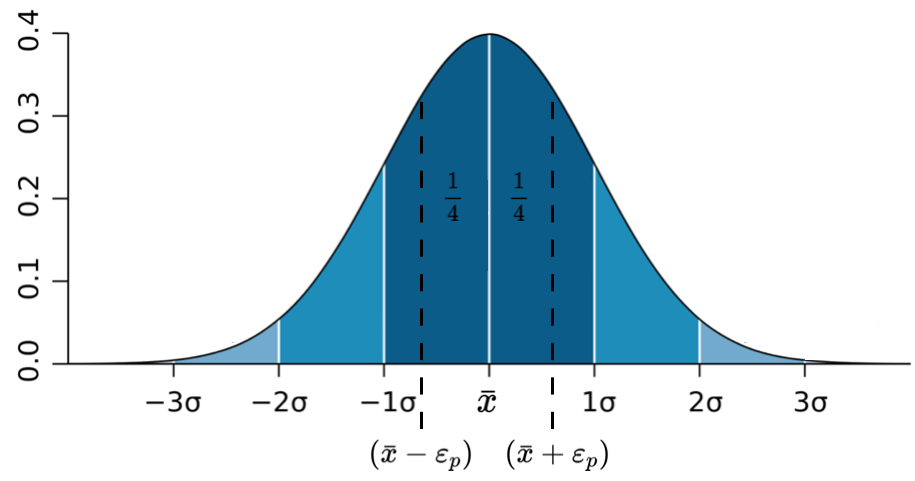
\includegraphics[height=2.1in,width=3.6in]{figuras/fig06}  
\caption{Curva de distribuci\'on de Gauss mostrando la posici\'on de $\bar{x}$ y $\sigma$}
\label{gauss5}
\end{center}
\end{figure}

Esto puede interpretarse diciendo que hay un $50 \%$ de probabilidad de que el valor verdadero se encuentre en ese intervalo. Para una distribuci\'on de Gauss, el error probable $\left(\varepsilon_p\right)$ est\'a dado por:
\begin{equation}
\varepsilon_p=0,674 \sigma
\end{equation}

El estudiante debe expresar en este caso, el resultado de una serie grande de medidas como:
\begin{equation}
x=\left(\bar{x} \pm \varepsilon_p\right) \quad \text {[unidades]} \,.
\end{equation}

La teor\'ia estad\'istica dice que de todas las medidas el:
\begin{itemize}
\item  $38,3 \%$ est\'an comprendidas en el intervalo de $\bar{x}-\frac{\sigma}{2}$ hasta $\bar{x}+\frac{\sigma}{2}$.
\item  $50,0 \%$ est\'an comprendidas en el intervalo de $\bar{x}-\varepsilon_p$ hasta $\bar{x}+\varepsilon_p$.
\item $68,3 \%$ est\'an comprendidas en el intervalo de $\bar{x}-\sigma$ hasta $\bar{x}+\sigma$.
\item $82,2 \%$ est\'an comprendidas en el intervalo de $\bar{x}-2 \varepsilon_p$ hasta $\bar{x}+2 \varepsilon_p$.
\item 95,45\% est\'an comprendidas en el intervalo de $\bar{x}-2 \sigma$ hasta $\bar{x}+2 \sigma$.
\item 95,69\% est\'an comprendidas en el intervalo de $\bar{x}-3 \varepsilon_p$ hasta $\bar{x}+3 \varepsilon_p$.
\item $99,73 \%$ est\'an comprendidas en el intervalo de $\bar{x}-3 \sigma$ hasta $\bar{x}+3 \sigma$.
\end{itemize}

\paragraph{Ejemplo 2.} Consideremos el siguiente conjunto de medidas que se corresponden a 25 medidas para el di\'ametro de un tubo, Tabla \ref{diametros2}. Para ese conjunto de valores tenemos:
\begin{table}[h]
\begin{center}
\begin{tabular}{|c|c|c|c|}
\hline   &  &  &  \\
 $\mathrm{N}^{\circ}$ \text {de medida} & $d(\mathrm{mm}$) & ($\bar{d}-d$) $\mathrm{~mm}$ & ($\Delta d)^2$ mm$^2$ \\
\hline \hline 1 & 15,12 & 0,016 & 0,0003 \\
\hline 2 & 15,10 & 0,036 & 0,0013 \\
\hline 3 & 15,15 & -0,014 & 0,0002 \\
\hline 4 & 15,17 & -0,034 & 0,0011 \\
\hline 5 & 15,14 & -0,004 & 0,00002 \\
\hline 6 & 15,16 & -0,024 & 0,0006 \\
\hline 7 & 15,14 & -0,004 & 0,0002 \\
\hline 8 & 15,12 & 0,016 & 0,0003 \\
\hline 9 & 15,12 & 0,016 & 0,0003 \\
\hline 10 & 15,14 & -0,004 & 0,00002 \\
\hline 11 & 15,15 & -0,014 & 0,0002 \\
\hline 12 & 15,14 & -0,004 & 0,00002 \\
\hline 13 & 15,13 & 0,006 & 0,00004 \\
\hline 14 & 15,14 & -0,004 & 0,00002 \\
\hline 15 & 15,13 & 0,006 & 0,00004 \\
\hline 16 & 15,13 & 0,006 & 0,00004 \\
\hline 17 & 15,14 & -0,004 & 0,00002 \\
\hline 18 & 15,14 & -0,004 & 0,00002 \\
\hline 19 & 15,14 & -0,004 & 0,00002 \\
\hline 20 & 15,13 & 0,006 & 0,00004 \\
\hline 21 & 15,15 & -0,014 & 0,0002 \\
\hline 22 & 15,13 & 0,006 & 0,00004 \\
\hline 23 & 15,15 & -0,014 & 0,0002 \\
\hline 24 & 15,11 & 0,026 & 0,0007 \\
\hline 25 & 15,13 & 0,006 & 0,00004 \\
\hline \text { Suma } & $\mathbf{3 7 8 , 4 0}$ & & $\mathbf{0 , 0 0 5 8}$ \\
\hline \text { Promedio } &$ \mathbf{1 5 , 1 3 6}$ & & \\
\hline
\end{tabular}
\end{center}
\caption{Medidas para di\'ametro $d$ de un tubo}
\label{diametros2}
\end{table}

\begin{itemize}
\item  La desviaci\'on est\'andar:
$$
\sigma=\sqrt{\frac{\sum_{i=1}^N(\Delta d)^2}{(N-1)}}=\sqrt{\frac{0,0058 \mathrm{~mm}^2}{24}}=0,02 \mathrm{~mm} .
$$
\item  Error probable:
$$
e_p=0,674 \times \sigma=0,01 \mathrm{~mm} .
$$
\item  Error relativo:
$$
\varepsilon_d=\frac{e_p}{\bar{d}}=\frac{0,01 \mathrm{~mm}}{15,14 \mathrm{~mm}}=7 \times 10^{-4} .
$$
\item  Error porcentual:
$$
\varepsilon_{\%}=\varepsilon_d \times 100=7 \times 10^{-4} \times 100=7 \times 10^{-2}=0,07 \% .
$$
\item  Valor del di\'ametro:
$$
d=(15,14 \pm 0,01) \mathrm{~mm} 
$$
\end{itemize}

Con Python podemos hacer los c\'alculos del Ejemplo 2, pero es bueno notar lo siguiente. Numpy tiene una funci\'on para calcular la desviaci\'on est\'andar que es {\bf std} que se basa en la ecuaci\'on 
$$
\sigma=\sqrt{\frac{\sum_{i=1}^N(d_i -\bar{d})^2}{N}}
$$
que ser\'ia la desviaci\'on est\'andar  no corregida de una muestra (considerada como la poblaci\'on total).
\begin{lstlisting}[language=Python]    
sig=std(d)
sig
\end{lstlisting}
\begin{tcolorbox}[width=\textwidth,colback={ghostwhite}]   
{\small 
0.014966629547095968 
}
\end{tcolorbox}

Pero aqu\'i estaremos utilizando la ecuaci\'on \ref{des1}  que tambi\'en se conoce como la desviaci\'on est\'andar de una muestra corregida. Esa diferencia entre $1/N$ y $1/(N-1)$ se hace cada vez m\'as peque\~na a medida que $N$ aumenta. Podemos definir nuestra propia desviaci\'on est\'andar.
\begin{lstlisting}[language=Python]    
des = sqrt(sum((d - mean(d))**2  )/(len(d)-1))
des
\end{lstlisting}
\begin{tcolorbox}[width=\textwidth,colback={ghostwhite}]   
{\small 
0.015275252316519673
}
\end{tcolorbox}

Para el resto de los c\'alculos del ejemplo 2 tenemos:
\begin{lstlisting}[language=Python]    
epr=(0.674*des)
ed=epr/mean(d)
ep=ed*100
print('promedio:', mean(d).round(2))
print('error probable:', epr.round(2))
print('error relativo:', ed.round(4))
print('error porcentual:', ep.round(2),'%')
\end{lstlisting}
\begin{tcolorbox}[width=\textwidth,colback={ghostwhite}]   
{\small 
promedio: 15.14 \\
error probable: 0.01 \\
error relativo: 0.0007 \\
error porcentual: 0.07 \%
}
\end{tcolorbox} 


\subsection{Precisi\'on y exactitud de mediciones}

Volviendo al tema de la precisi\'on y exactitud de las mediciones vimos que est\'an relacionadas con los errores co�metidos en la obtenci\'on de las mismas. La precisi\'on en el valor medio es proporcional al inverso del error casual o estad\'is�tico. Se obtendr\'a una alta precisi\'on si el error (porcentual) estad\'istico es peque\~no y ser\'a baja si dicho error es grande. La exactitud ser\'a alta cuando los errores sistem\'aticos sean peque\~nos y ser\'a baja si \'estos son grandes.

En algunos casos, una alta exactitud puede implicar un error casual peque\~no, pero
en general no es as\'i. La precisi\'on y exactitud no son t\'erminos intercambia�bles entre s\'i y los m\'etodos estad\'isticos dan espec\'ificamente una medida cuantita�tiva de la precisi\'on y no de la exactitud.

Las diferencias entre exactitud y precisi\'on se ilustran en la figura \ref{gauss4}. En la figura de la izquierda se observa que el valor medio difiere bastante del valor verdadero, lo cual se interpreta diciendo que las mediciones fueron de baja exactitud, la gaussiana $B$  indica una baja exactitud y una alta precisi\'on.
\begin{figure}[h]
\begin{center}
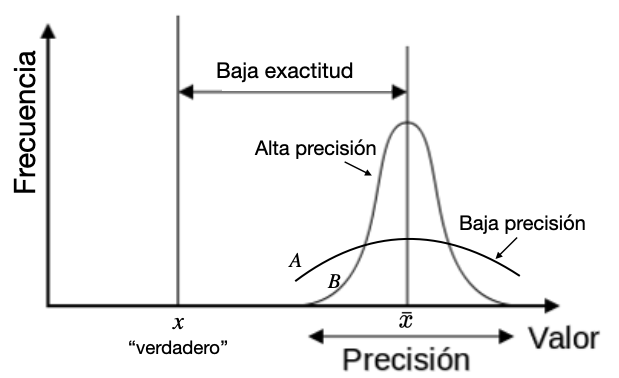
\includegraphics[height=2.1in,width=3.2in]{figuras/fig07a}  
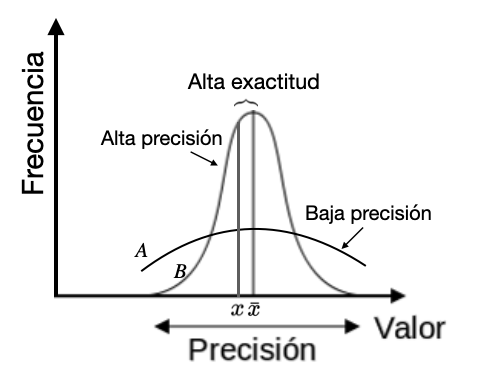
\includegraphics[height=2.1in,width=3.0in]{figuras/fig07b}  
\caption{Precisi\'on y Exactitud}
\label{gauss4}
\end{center}
\end{figure}

En la misma figura pero de la derecha, en la gausiana ${B}$, el intervalo $\left(\bar{x}-\varepsilon_p, \bar{x}+\varepsilon_p\right)$ es menor que en la gaussiana $A$, por lo tanto las mediciones que corresponden a la gaussiana $B$ son de mayor precisi\'on y una alta exactitud.

\subsection{Discrepancia}
Cuando tenemos dos mediciones de una misma cantidad, por ejemplo
$$
x_1=\left(x_{01} \pm \Delta x_1\right) \quad \text{y}\quad 
x_2=\left(x_{02} \pm \Delta x_2\right)
$$
decimos que tenemos una discrepancia si estas mediciones no coinciden.

Definimos la discrepancia entre dos medidas como la diferencia entre las  medidas de la misma cantidad:
$$
\text { Discrepancia}= \mathcal{D}=\left|x_{01}-x_{02}\right| 
$$

No es exactamente un error pero es una cantidad que puede ser significativa para el c\'alculo de los errores.

Por ejemplo, dos estudiantes miden las siguientes temperaturas en un experimento:
$$
T_A=(2,2 \pm 0,1) \mathrm{~K} \,, \quad T_B=(2,7 \pm 0,2) \mathrm{~K} \,\, \Rightarrow \,\, 
\mathcal{D}=\left|2.2-2.7\right| = 0,5
$$
Lo anterior es igual a:
$$
2,1 \leq T_A \leq 2,3  \mathrm{~K} \quad \text{y} \quad 2,5 \leq  T_B \leq 2,9  \mathrm{~K}
$$
y se dice  que ambas mediciones son distinguibles entre s\'i porque los intervalos no se solapan.

Pero resulta que otros dos estudiantes miden las siguientes temperaturas
$$
T_A=(2,3 \pm 0,1) \mathrm{~K}\,, \quad T_B=(2,5 \pm 0,2) \mathrm{~K} \,\, \Rightarrow \,\, 
\mathcal{D}=\left|2.3-2.5\right| = 0,2
$$
que es equivalente  a:
$$
2,2 \leq T_A \leq 2,4  \mathrm{~K} \quad \text{y} \quad   2,3 \leq  T_B \leq 2,7  \mathrm{~K}
$$
en este caso,  la discrepancia es de 0,2  pero no es significativa porque los intervalos de las mediciones se superponen, decimos entonces que las mediciones son indistinguibles.

Podemos hablar de una discrepancia porcentual si tomamos la media de las medidas, para el primer caso el promedio de las dos medidas es: 2,45 K.
$$
\mathcal{D}_{\%}= \left|\frac{0,5}{2,45}\right| \times 100 = 20 \%
$$

Y para el segundo par de medidas el promedio es 2,4 K
$$
\mathcal{D}_{\%}= \left|\frac{0,2}{2,4}\right| \times 100 = 8 \%
$$


\section{Algoritmo para el manejo de los errores}

Podemos crear un algoritmo que nos ayude a definir los criterios que debemos utilizar a la hora de escribir los resultados de las mediciones hechas en el laboratorio. Para darle a nuestras mediciones una validez estad\'istica es conveniente realizar el calculo de la dispersi\'on $D$, ecuaci\'on \ref{disper}, la dispersi\'on porcentual \ref{disperpor} y  tener a mano la sensibilidad $S$ del aparato de medida.

Realicemos los siguientes pasos
\begin{enumerate}
\item Tomaremos $N=3$ mediciones como el valor m\'inimo para nuestro algoritmo.
\begin{description}
\item[i) Si $D < S$:]  El error vendr\'a dado por $\Delta x= S$ y la medida es $\bar{x}_3$, por lo tanto
$$
\mathrm{M}= \bar{x}_3  \pm  S \quad \mathrm{[Unidades]} 
$$
\item [ii) Si  $D > S$ y $D_{\%} \leq 2\%$:]  El error vendr\'a dado por $\Delta x= S$ y la medida es $\bar{x}_3$
$$
\mathrm{M}= \bar{x}_3 \,  \pm \, S \quad \mathrm{[Unidades]} 
$$
\end{description}
donde 
$$
\bar{x}_3=\frac{1}{3}{\sum_{i=1}^3 x_i}
$$

\item Si para $N=3$ se tiene que $D > S$ pero la dispersi\'on est\'a entre: $2\% \leq D_{\%} \leq 8\% $, entonces  realizamos m\'as medidas hasta llegar a  $N=6$.  El error vendr\'a dada por el valor m\'aximo entre $D_6/4$ y $S$, donde $D_6$ es la dispersi\'on para 6 medidas, es decir:
$$
\mathrm{M}= \bar{x}_6 \,  \pm \,  \mathrm{max} \left\{D_6 /4, S \right\}  \quad \mathrm{[Unidades]} 
$$
donde
$$
\bar{x}_6=\frac{1}{6}{\sum_{i=1}^6 x_i}
$$

\item Si para $N=3$ se tiene que $D > S$ pero la dispersi\'on est\'a entre: $8\% \leq D_{\%} \leq 15\% $, entonces  hacemos $N=15$, y el error vendr\'a dado por
$$
\Delta x_{15}=\sqrt{\frac{\sum_{i=1}^{15}\left(x_i-\bar{x}_{15}\right)^2}{14}}
$$
La magnitud se escribe entonces como 
$$
\mathrm{M}= \bar{x}_{15}  \pm \Delta x_{15}   \quad \mathrm{[Unidades]} 
$$
donde
$$
\bar{x}_{15}=\frac{1}{15}{\sum_{i=1}^{15} x_i}
$$

\item  Si para $N=3$ se tiene que $D > S$ per la dispersi\'on es $ D_{\%} \geq 15\% $, entonces demos hacer muchas medidas $N \geq 50$, y el error vendr\'a dado por
$$
\Delta x_{N}=\sqrt{\frac{\sum_{i=1}^N\left(x_i-\bar{x}_N\right)^2}{N(N-1)}}
$$
La magnitud se escribe entonces como 
$$
\mathrm{M}= \bar{x}_{N}  \pm \Delta x_{N}   \quad \mathrm{[Unidades]} 
$$
donde 
$$
\bar{x}_{N}=\frac{1}{N}{\sum_{i=1}^{N} x_i} \,.
$$

Notemos que si  por ejemplo, se ha obtenido que $D > S$ y $2\% \leq D_{\%} \leq 8\% $ se necesitan  6 medidas y el valor verdadero queda establecido en la media aritm\'etica de las 6 medidas y su error corresponde al m\'aximo de entre la dispersi\'on de las seis medidas dividido por 4 o la sensibilidad.

Por otro lado, si se realizan 15 o m\'as medidas, en realidad se est\'a buscando que el conjunto de las mismas sea una distribuci\'on gaussiana o normal, en cuyo caso, el error que se considera corresponde con el error cuadr\'atico medio (ECM) o desviaci\'on standard $\sigma$. 
\end{enumerate}

\paragraph{Ejemplo 3.} Con una regla graduada, en mil\'imetros, se mide la longitud $L$ de un tubo. El error de cada medida para este instrumento anal\'ogico es
$$
\varepsilon_p= \frac{1\mathrm{~mm}}{2}= 0,5 \mathrm{~mm} =S 
$$

\begin{itemize}
\item Los datos obtenidos para tres medidas son:
$$
\begin{array}{|c|c|c|c|}
\hline \hline 
L (\mathrm{mm}) &15,0 & 14,0 & 13,5 \\
\hline 
\end{array}
$$
La media:
$$
\bar{L}= \frac{15,0 + 14,0 + 13,5}{3}= \frac{42,5}{3}= 14,2 \mathrm{~mm}
$$
La dispersi\'on para estos datos es de
$$
D=15,0 - 13,5 = 1,5 \,\, \Rightarrow \,\, D_{\%}= \frac{1,5}{14,2} \cdot 100  = 11 \%
$$

Estamos en el caso donde  $D > S$  y la dispersi\'on porcentual resulta ser mayor al $2\%$. Debemos hacer m\'as medidas

\item Agregamos tres medidas m\'as para completar 6 mediciones
$$
\begin{array}{|c|c|c|c|c|c|c|}
\hline \hline 
L (\mathrm{mm}) &15,0 & 14,0 & 13,5 & 15,5&15,5 & 15,5\\
\hline 
\end{array}
$$
La media:
$$
\bar{L}=\frac{15,0 + 14,0 + 13,5+15,5+15,5 + 15,5}{6}= \frac{89,0}{6}= 14,8 \mathrm{~mm}
$$
La dispersi\'on para estos datos es ahora de 
$$
D=15,5 - 13,5 = 2,0 \,\,\Rightarrow \,\, D_{\%}= \frac{2,0}{14,8} \cdot 100  = 14 \%
$$
Con $N=6$, nuevamente tenemos que $D > S$  y la dispersi\'on porcentual se encuentra fuera del rango $2\% \leq D_{\%} \leq 8\% $. Debemos tomar m\'as medidas. 

\item Agregamos 9 medidas m\'as para completar $N=15$
$$
\begin{array}{ccc}
\hline \hline L(\mathrm{~mm}) & L(\mathrm{~mm}) & L(\mathrm{~mm}) \\\hline 
15,0 & 14,0 & 13,5 \\
15,5 & 15,5 & 15,5 \\
13,5 & 15,0 & 14,0 \\
14,0 & 14,0 & 15,5 \\
13,5 & 14,0 & 14,0 \\
\hline \hline
\end{array}
$$
La media:
$$
\bar{L}=\frac{1}{15}{\sum_{i=1}^{15} L_i} = \frac{216}{15}= 14,4 \mathrm{~mm}
$$
La dispersi\'on para estos datos es ahora de 
$$
D=15,5 - 13,5 = 2,0 \,\Rightarrow \, D_{\%}= \frac{2,0}{14,4} \cdot 100  = 14 \%
$$

Con $N=15$, nuevamente tenemos que $D > S$  pero ahora la dispersi\'on porcentual se encuentra dentro del rango $8\% \leq D_{\%} \leq 15\% $. Podemos parar y proceder a calcular los errores completando la  siguiente tabla
$$
\begin{array}{|c|c|c|c|}
\hline i & L_i \pm 0,5  (\mathrm{mm}) & L_i-\bar{L} (\mathrm{mm}) & \left(L_i-\bar{L}\right)^2 (\mathrm{mm}^2) \\\hline 
1 & 15,0 & 0,6 & 0,36 \\
2 & 15,5 & 1,1 & 1,21 \\
3 & 13,5 & -0,9 & 0,81 \\
4 & 14,0 & -0,4 & 0,16 \\
5 & 13,5 & -0,9 & 0,81 \\
6 & 14,0 & -0,4 & 0,16 \\
7 & 15,5 & 1,1 & 1,21 \\
8 & 15,0 & 0,6 & 0,36 \\
9 & 14,0 & -0,4 & 0,16 \\
10 & 14,0 & -0,4 & 0,16 \\
11 & 13,5 & -0,9 & 0,81 \\
12 & 15,5 & 1,1 & 1,21 \\
13 & 14,0 & -0,4 & 0,16 \\
14 & 15,5 & 1,1 & 1,21 \\
15 & 14,0 & -0,4 & 0,16 \\
\hline \sum & 216 & & 8,95 \\
\hline
\end{array}
$$

Por lo tanto:
$$
\Delta x_{15}=\sqrt{\frac{\sum_{i=1}^{15}\left(L_i-\bar{L}_{15}\right)^2}{14}}=\sqrt{\frac{8,95}{14}} =0,214  \mathrm{~mm}
$$

La longitud L del tubo  se escribe entonces como 
$$
L= 14,4  \pm 0,2  \mathrm{~mm}
$$

\end{itemize}





\section{Mediciones indirectas}
Hasta aqu\'i se ha analizado lo correspondiente a errores de magnitudes medidas directamente, por ejemplo: la altura de un cilindro, el di\'ametro de un tubo, el tiempo de ca\'ida de un cuerpo. Frecuentemente la magnitud de inter\'es debe ser determinada a partir de otras magnitudes medidas directamente, por lo que el error en dicha magnitud debe ser obtenido a partir de los errores de las otras magnitudes.

Por ejemplo, para la determinar el volumen $V$ de un cilindro se efect\'uan medidas del di\'ametro $d$ y la altura $h$, luego el error en $V$ debe ser obtenido de los errores cometidos en las medidas de $d$ y $h$.  El procedimiento que permite obtener este error es lo que se conoce como propagaci\'on de errores.

\subsection{Propagaci\'on de errores}
Como indicamos anteriormente, la medida indirecta de una magnitud se alcanza por aplicaci\'on de una f\'ormula a un conjunto de medidas directas, (las variables independientes o los datos), que las relacionan con la magnitud del problema. Mediante dicha f\'ormula se puede obtener tambi\'en el error de la medida. 

\subsection{Propagaci\'on de errores en casos particulares}

A continuaci\'on analizaremos algunos de los casos m\'as sencillos de propagaci\'on de errores:

\paragraph{Suma y diferencia de magnitudes.}

Cuando una magnitud M es el resultado de la suma o resta de dos o m\'as magnitudes medidas directamente, un error en dichas magnitudes traer\'a consigo un error en M, es decir, si $(X \pm \Delta X)$ y $(Y \pm \Delta Y)$ son dos mediciones directas, entonces 
$$
\mathrm{M}=X  \pm Y \,\, \Rightarrow \,\, \mathrm{M} \pm \Delta \mathrm{M}=(X \pm \Delta X) \pm(Y \pm \Delta Y) \,,
$$
reagrupando t\'erminos resulta,
$$
\mathrm{M} \pm \Delta \mathrm{M}=(X \pm Y) \pm(\Delta X+\Delta Y)
$$
donde
$$
\Delta \mathrm{M}=\Delta X+\Delta Y
$$

El error absoluto $\Delta$M, de la suma o diferencia de magnitudes, viene dado por la suma de los errores absolutos de cada una de las magnitudes medidas directamente.

El error relativo ser\'a:
$$
\varepsilon_r=\frac{\Delta \mathrm{M}}{\mathrm{M}}=\frac{\Delta X+\Delta Y}{X \pm Y}
$$

\paragraph{Multiplicaci\'on de magnitudes.} 
Si la magnitud M es el resultado de multiplicar dos o m\'as magnitudes medidas en forma directa, el error absoluto $\Delta$M se puede obtener de la siguiente manera:
$$
\mathrm{M}  =X \cdot Y \,\, \Rightarrow \,\,  \mathrm{M} \pm \Delta\mathrm{M}  =(X \pm \Delta X) \cdot (Y \pm \Delta Y)  \,,
$$
por lo tanto
$$
\mathrm{M} \pm \Delta \mathrm{M}  =(X \cdot Y) \pm X \Delta Y \pm Y \Delta X+\Delta X \Delta Y \,.
$$

Puesto que las cantidades $\Delta X$ y $\Delta Y$ son peque\~nas comparadas con $X$ y $Y$, se puede despreciar el t\'ermino $\Delta X \Delta Y$ y el error absoluto de $M$ ser\'a:
$$
\Delta \mathrm{M}=X \Delta Y+Y \Delta X \,.
$$

El error relativo:
$$
\varepsilon_r=\frac{\Delta \mathrm{M}}{\mathrm{M}}=\frac{\Delta X}{X}+\frac{\Delta Y}{Y}
$$
es decir, el error relativo de un producto de magnitudes es la suma de los errores relativos de cada una de las magnitudes medidas directamente.

\paragraph{Divisi\'on de magnitudes.} 
Cuando la magnitud M es el resultado de dividir magnitudes medidas directamente, el error absoluto se puede obtener en la forma siguiente:
$$
\mathrm{M} =\frac{X}{Y} \,\, \Rightarrow \,\,  \mathrm{M} \pm \Delta \mathrm{M}  =\frac{X \pm \Delta X}{Y \mp \Delta Y} \,,
$$
por lo tanto:
$$
\mathrm{M} \pm \Delta \mathrm{M}  =\frac{X \pm \Delta X}{Y \mp \Delta Y} \cdot \frac{Y \pm \Delta Y}{Y \pm \Delta Y} =\frac{X Y \pm Y \Delta X \pm X \Delta Y+\Delta X \Delta Y}{Y^2-(\Delta Y)^2} \,.
$$

Considerando que $\Delta X$ y $\Delta Y$ son peque\~nos en relaci\'on a $X$ y $Y$, se puede despreciar los t\'erminos $\Delta X \Delta Y$ y $(\Delta Y)^2$, luego
$$
\mathrm{M} \pm \Delta\mathrm{M}=\frac{X}{Y} \pm \frac{Y \Delta X+X \Delta Y}{Y^2}\,,
$$
es decir, el error absoluto en M ser\'a:
$$
\Delta \mathrm{M}=\frac{Y \Delta X+X \Delta Y}{Y^2} \,,
$$
y el error relativo:
$$
\varepsilon_r=\frac{\Delta \mathrm{M}}{\mathrm{M}}=\frac{\Delta X}{X}+\frac{\Delta Y}{Y}\,.
$$

Al igual que para el producto de magnitudes, el error relativo del cociente es igual a la suma de los errores relativos de cada una de las magnitudes medidas directamente.


\paragraph{Funci\'on potencial.}
Si la magnitud M es el resultado de elevar la magnitud $X$ a una potencia $n$, M$=a X^n$, donde $a$ es un valor exacto. El error relativo se puede obtener aplicando el criterio definido para el producto de magnitudes.

Ya que M se puede escribir como:
$$
\mathrm{M}=a \cdot \underbrace{X \cdot X \cdot X \ldots  X}_{n \text { veces }}
$$
su error relativo ser\'a:
$$
\varepsilon_r=\frac{\Delta \mathrm{M}}{\mathrm{M}}=\underbrace{\frac{\Delta X}{X}+\frac{\Delta X}{X}+\ldots+\frac{\Delta X}{X}}_{n \text { veces }}
$$
luego
$$
\varepsilon_r=\frac{\Delta \mathrm{M}}{\mathrm{M}}=n \frac{\Delta X}{X}
$$
as\'i que, el error absoluto ser\'a:
$$
\Delta \mathrm{M}=a n X^{n-1} \Delta X \,.
$$

\subsection{Propagaci\'on de errores en casos generales}

En el caso en que la magnitud a determinar dependa de m\'as de dos magnitudes medidas directamente y relacionadas a trav\'es de diferentes operaciones matem\'aticas, el c\'alculo del error absoluto y del relativo se puede realizar por uno de los m\'etodos siguientes:

\subsubsection{M\'etodo del binomio}

Consideremos un caso en que la expresi\'on que relaciona la magnitud M con las magnitudes $X, Y, Z$ y $T$ sea del tipo:
$$
\mathrm{M}=\frac{X^a  Y^b}{Z^c  T^d}=X^a  Y^b  Z^{-c}  T^{-d}
$$

Para la obtenci\'on del error en M, supongamos que el experimento sea tan desafortunado que todos los errores influyan en el resultado en la misma direcci\'on. En este caso el m\'aximo error posible en $\mathrm{M}$ vendr\'a dado por:
$$
\begin{aligned}
\mathrm{M} \pm \Delta \mathrm{M} & =\frac{(X+\Delta X)^a (Y+\Delta Y)^b}{(Z-\Delta Z)^c  (T-\Delta T)^d}  =(X+\Delta X)^a (Y+\Delta Y) (Z-\Delta Z)^{-c} (T-\Delta T)^{-d}
\end{aligned}
$$

Esto suceder\'a si los valores de $X$ y $Y$ son grandes, mientras que los de $Z$ y $T$ son peque\~nos. La expresi\'on anterior puede ser escrita en la forma siguiente:
$$
\mathrm{M} \left(1+\frac{\Delta \mathrm{M}}{\mathrm{M}}\right)=X^a Y^b Z^{-c} T^{-d} \left(1+\frac{\Delta X}{X}\right)^a\left(1+\frac{\Delta Y}{Y}\right)^b\left(1-\frac{\Delta Z}{Z}\right)^{-c}\left(1-\frac{\Delta T}{T}\right)^{-d}
$$
luego,
$$
\left(1+\frac{\Delta \mathrm{M}}{\mathrm{M}}\right)=\left(1+\frac{\Delta X}{X}\right)^a\left(1+\frac{\Delta Y}{Y}\right)^b\left(1-\frac{\Delta Z}{Z}\right)^{-c}\left(1-\frac{\Delta T}{T}\right)^{-d}
$$

Si suponemos que los errores absolutos son peque\~nos comparados con las magnitudes medidas, los t\'erminos, $\frac{\Delta X}{X}, \frac{\Delta Y}{Y}, \frac{\Delta Z}{Z}$ y $\frac{\Delta T}{T}$ son a\'un m\'as peque\~nos, por consiguiente al desarrollar cada uno de los binomios de Newton y despreciar los t\'erminos elevados al cuadrado o de potencias mayores, lo que queda es:
$$
\left(1+\frac{\Delta \mathrm{M}}{\mathrm{M}}\right) \simeq\left(1+a \frac{\Delta X}{X}\right) \left(1+b \frac{\Delta Y}{Y}\right) \left(1+c \frac{\Delta Z}{Z}\right) \left(1+d \frac{\Delta T}{T}\right)
$$

Efectuando las multiplicaciones y despreciando los productos de los t\'erminos peque\~nos, se tiene:
\begin{equation}
\varepsilon_r=\frac{\Delta \mathrm{M}}{\mathrm{M}}=a \frac{\Delta X}{X}+b \frac{\Delta Y}{Y}+c \frac{\Delta Z}{Z}+d \frac{\Delta T}{T}
\label{binomio}
\end{equation}
es decir, el error relativo de M corresponde a la suma de los errores relativos de cada magnitud multiplicados por sus exponentes respectivos.

Si se multiplica por 100 la expresi\'on anterior, se obtiene el error porcentual en $M$ como funci\'on de los porcentajes de error que introducen cada una de las magnitudes:
$$
\varepsilon_{\%}=a \varepsilon_{X\%}+b \varepsilon_{Y\%}+c \varepsilon_{Z\%}+d \varepsilon_{T\%} \,.
$$

\paragraph{Ejemplo 4.} Supongamos que una magnitud M est\'a relacionada con las magnitudes: $X_1, X_2, Y, Z, T_1$ y $T_2$, mediante una expresi\'on del tipo:
\begin{equation}
\mathrm{M}=\frac{\left(X_1+X_2\right)  Y^2}{Z\left(T_1-T_2\right)^3} \,.
\label{eme3}
\end{equation}

Para utilizar la expresi\'on (\ref{binomio}), se debe llevar la expresi\'on M a una forma que contenga s\'olo productos y/o cocientes de magnitudes. Para lograr esto, se realiza el siguiente cambio de variables,
\begin{equation}
\begin{aligned}
X & =X_1+X_2 \\
T & =T_1-T_2
\end{aligned}
\label{camva}
\end{equation}

Como $X$ y $T$ son el resultado de una suma y una resta, respectivamente, se sabe que el error absoluto de cada una de ellas viene dado por:
$$
\begin{aligned}
\Delta X & =\Delta X_1+\Delta X_2 \\
\Delta T & =\Delta T_1+\Delta T_2
\end{aligned}
$$
Usando (\ref{camva}) M se puede expresar como:
$$
\mathrm{M}=\frac{X  Y^2}{Z  T^3}
$$
De acuerdo a la expresi\'on (\ref{binomio}), el error relativo de M ser\'a:
$$
\varepsilon_r=\frac{\Delta \mathrm{M}}{\mathrm{M}}=\frac{\Delta X}{X}+2 \frac{\Delta Y}{Y}+\frac{\Delta Z}{Z}+3 \frac{\Delta T}{T} \,.
$$


\paragraph{Ejemplo 5.} Para calcular los errores en el volumen del cilindro estudiado anteriormente, (Ejemplo 1) se har\'a uso de la expresi\'on (\ref{binomio}).

Con los valores medidos de $h= (10,2 \pm 0,1)$ cm y $d=(1,784 \pm 0,005)$ cm, el volumen del cilindro estar\'a dado por:
$$
V=\pi r^2 h=\frac{\pi d^2 h}{4}=\frac{\pi (1,784)^2  (10,2)}{4}= 25,5 \mathrm{~cm}^3 \,.
$$

El error relativo ser\'a:
$$
\varepsilon_r=\frac{\Delta V}{V}=2 \frac{\Delta D}{D}+\frac{\Delta h}{h}=2 \cdot (0,0028)+0,01=0,016 \,.
$$
El error porcentual,
$$
\varepsilon_{\%}=\varepsilon_r \cdot 100=0,016 \cdot 100=1,6 \simeq 2 \% \,.
$$
El error absoluto,
$$
\Delta V=0,016 \cdot V=0,4 \mathrm{~cm}^3\,,
$$
luego el valor calculado de $V$ se escribe de la siguiente manera:
$$
V=(25,5 \pm 0,4) \mathrm{cm}^3
$$

Nota: El error absoluto de la magnitud f\'isica se escrib\'io con una cifra significativa. Esto condiciona el n\'umero de cifras significativa del valor de la magnitud.

\subsubsection{M\'etodo de las derivadas parciales}
Existe un m\'etodo alternativo al dado anteriormente para la propagaci\'on de errores, el cual hace uso de las derivadas y que explicaremos a continuaci\'on.

Sea una magnitud M, la cual es funci\'on de las magnitudes independientes $X, Y, Z, T, \ldots$
$$
\mathrm{M}=\mathrm{M}(X, Y, Z, T, \ldots)
$$

El error en M es producido por cada uno de los errores de las magnitudes $X, Y, Z, T, \ldots$, independientemente uno de los otros. A estos errores se les llama errores parciales y la suma de ellos, considerando el caso m\'as desfavorable, dar\'a el error en M.

El error absoluto en M estar\'a dado por:
\begin{equation}
\Delta \mathrm{M}=\left|\frac{\partial \mathrm{M}}{\partial X}\right||\Delta X|+\left|\frac{\partial \mathrm{M}}{\partial Y}\right||\Delta Y|+\left|\frac{\partial \mathrm{M}}{\partial Z}\right||\Delta Z|+\left|\frac{\partial \mathrm{M}}{\partial T}\right||\Delta T|+\ldots
\end{equation}
donde los t\'erminos $\frac{\partial \mathrm{M}}{\partial X}, \frac{\partial \mathrm{M}}{\partial Y}, \frac{\partial \mathrm{M}}{\partial Z}, \frac{\partial \mathrm{M}}{\partial T}, \ldots$ son las derivadas de M con respecto a $X, Y, Z, T, \ldots$, respectivamente. 

Estas se determinan derivando la funci\'on M con respecto a cada una de las variables en forma separada y considerando constantes las dem\'as, es decir, al derivar M con respecto a $X$ se considera a las variables $Y, Z, T, \ldots$ como constantes, y as\'i sucesivamente cuando se deriva respecto a $Y$, \'o a $Z, \ldots$

El error relativo se determina como el cociente entre el error absoluto y la funci\'on misma.
\begin{equation}
\varepsilon_{\mathrm{r}}=\frac{\Delta \mathrm{M}}{\mathrm{M}}=\frac{1}{\mathrm{M}(X, Y, Z, T, \ldots)}\left\{\left|\frac{\partial \mathrm{M}}{\partial X}\right||\Delta X|+\left|\frac{\partial \mathrm{M}}{\partial Y}\right||\Delta Y|+\left|\frac{\partial \mathrm{M}}{\partial Z}\right||\Delta Z|+\left|\frac{\partial \mathrm{M}}{\partial T}\right||\Delta T|+\ldots\right\}
\end{equation}

\paragraph{Ejemplo 6.}

Obtendremos el error relativo para la expresi\'on (\ref{eme3}) del ejemplo 3, utilizando el m\'etodo de las derivadas parciales:
$$
\mathrm{M}=\frac{\left(X_1+X_2\right)  Y^2}{Z \left(T_1-T_2\right)^3}
$$
Las derivadas parciales de M respecto a cada una de las variables son las siguientes:
\begin{eqnarray*}
\frac{\partial \mathrm{M}}{\partial X_1}&=&\frac{Y^2}{Z\left(T_1-T_2\right)^3}\,, \quad 
\frac{\partial \mathrm{M}}{\partial X_2}=\frac{Y^2}{Z\left(T_1-T_2\right)^3}\,, \quad
\frac{\partial \mathrm{M}}{\partial Y}=\frac{2 Y\left(X_1+X_2\right)}{Z\left(T_1-T_2\right)^3}\,\\
\frac{\partial \mathrm{M}}{\partial Z}&=&-\frac{\left(X_1+X_2\right)Y^2}{Z^2\left(T_1-T_2\right)^3} \,,\quad  \frac{\partial \mathrm{M}}{\partial T_1}=-\frac{3\left(X_1+X_2\right) Y^2}{Z\left(T_1-T_2\right)^4} \,,\quad \frac{\partial \mathrm{M}}{\partial T_2}=\frac{3\left(X_1+X_2\right) Y^2}{Z\left(T_1-T_2\right)^4}
\end{eqnarray*}

El error absoluto ser\'a:
$$
\Delta \mathrm{M}=\left|\frac{\partial \mathrm{M}}{\partial X_1}\right|\left|\Delta X_1\right|+\left|\frac{\partial \mathrm{M}}{\partial X_2}\right|\left|\Delta X_2\right|+\left|\frac{\partial \mathrm{M}}{\partial Y}\right||\Delta Y|+\left|\frac{\partial \mathrm{M}}{\partial Z}\right||\Delta Z|+\left|\frac{\partial \mathrm{M}}{\partial T_1}\right|\left|\Delta T_1\right|+\left|\frac{\partial \mathrm{M}}{\partial T_2}\right|\left|\Delta T_2\right|\,.
$$
Por lo tanto
$$
\begin{aligned}
\Delta \mathrm{M} & =\frac{Y^2}{Z\left(T_1-T_2\right)^3} \Delta X_1+\frac{Y^2}{Z\left(T_1-T_2\right)^3} \Delta X_2+\frac{2 Y\left(X_1+X_2\right)}{Z\left(T_1-T_2\right)^3} \Delta Y  \\
& +\frac{\left(X_1+X_2\right) Y^2}{Z^2\left(T_1-T_2\right)^3} \Delta Z+\frac{3\left(X_1+X_2\right) Y^2}{Z\left(T_1-T_2\right)^4} \Delta T_1+\frac{3\left(X_1+X_2\right) Y^2}{Z\left(T_1-T_2\right)^4} \Delta T_2
\end{aligned}
$$
Simplificando:
$$
\begin{aligned}
\Delta \mathrm{M} & =\frac{Y^2\left(\Delta X_1+ \Delta X_2\right)}{Z\left(T_1-T_2\right)^3}  + \frac{Y\left(X_1+X_2\right)}{Z\left(T_1-T_2\right)^3} \left[{2\Delta Y}+\frac{Y\Delta Z}{Z}  \right]  \\
&+ \frac{3\left(X_1+X_2\right) Y^2 \left(\Delta T_1+ \Delta T_2\right)}{Z\left(T_1-T_2\right)^4} 
\end{aligned}
$$

El error relativo:
$$
\begin{aligned}
& \varepsilon_{\mathrm{r}}=\frac{\Delta \mathrm{M}}{\mathrm{M}}  = \frac{Z \left(T_1-T_2\right)^3}{\left(X_1+X_2\right)  Y^2} 
\left\{ \frac{Y^2\left(\Delta X_1+ \Delta X_2\right)}{Z\left(T_1-T_2\right)^3}  + \frac{Y\left(X_1+X_2\right)}{Z\left(T_1-T_2\right)^3} \left[{2\Delta Y}+\frac{Y\Delta Z}{Z}  \right]     \right. \\
& \left.+  \frac{3\left(X_1+X_2\right) Y^2 \left(\Delta T_1+ \Delta T_2\right)}{Z\left(T_1-T_2\right)^4} \right\} \\
\end{aligned}
$$
simplificamos nuevamente y finalmente  obtenemos
\begin{equation}
\frac{\Delta \mathrm{M}}{\mathrm{M}}=\frac{\Delta X_1+\Delta X_2}{X_1+X_2}+2 \frac{\Delta Y}{Y}+\frac{\Delta Z}{Z}+3 \frac{\Delta T_1+\Delta T_2}{T_1-T_2}
\end{equation}

Vemos que la expresi\'on anterior para el error relativo coincide con la obtenida  por el m\'etodo del binomio del ejemplo 4. Se debe notar que el m\'etodo de las derivadas es m\'as laborioso y necesita del conocimiento de las derivadas parciales. Sin embargo, este \'ultimo m\'etodo es aplicable a cualquier expresi\'on, mientras que el m\'etodo del binomio s\'olo es valido para expresiones que contengan solamente variables independientes.

Para ilustrar esto \'ultimo obtengamos el error relativo para la expresi\'on:
$$
\mathrm{M}=\frac{(a+z)^2}{(b+z)^2}
$$
donde $a$ y $b$ son constantes exactas.
\begin{description}
\item[a)]  M\'etodo del binomio

Primero realizaremos el siguiente cambio de variables:
\begin{itemize}
\item  $A=a+z \Rightarrow \Delta A=\Delta z$
\item  $B=b+z \Rightarrow \Delta B=\Delta z$
\end{itemize}

Note que las variables $A$ y $B$ son dependientes. Por lo tanto:
$$
\mathrm{M}=\frac{A^2}{B^2}
$$
para el error relativo se tendr\'a,
$$
\frac{\Delta \mathrm{M}}{\mathrm{M}}=2 \frac{\Delta A}{A}+2 \frac{\Delta B}{B}
$$
de aqu\'i,
$$
\begin{aligned}
\frac{\Delta \mathrm{M}}{\mathrm{M}} & =2 \frac{\Delta z}{a+z}+2 \frac{\Delta z}{b+z}  =\frac{2 a+2 b+4 z}{(a+z)(b+z)} \Delta z
\end{aligned}
$$

\item[b)]  M\'etodo de las derivadas parciales
$$
\Delta \mathrm{M}  =\left|\frac{\partial \mathrm{M}}{\partial z}\right||\Delta z| 
$$
donde
$$
\frac{\partial \mathrm{M}}{\partial z}  =\frac{2(a+z)(b+z)-2(a+z)^2}{(b+z)^3}
$$
Por lo tanto
$$
\frac{\Delta \mathrm{M}}{\mathrm{M}}  =\frac{(b+z)^2}{(a+z)^2}\left\{\frac{2(a+z)(b+z)-2(a+z)^2}{(b+z)^3}\right\} \Delta z  =\frac{2(b-a)}{(a+z)(b+z)} \Delta z
$$
\end{description}
Como se puede ver, se ha obtenido dos expresiones diferentes para el error en M; sin embargo, s\'olo una de ellas es correcta. Analicemos el caso particular en que $a=b$ entonces se tendr\'a que M=1, eso implica que el error relativo de M debe ser cero.

Lo anterior muestra que el m\'etodo de las derivadas parciales da el resultado correcto para el error en M.

\paragraph{Nota:} si en las ecuaciones aparecen n\'umeros irracionales: $\pi$, $e$, $\gamma...$ es necesario tomar en cuenta un n\'umero de cifras significativas que no afecte a la magnitud del error absoluto de la cantidad que queremos determinar. Como lo m\'as probable es que estos valores se obtengan de un ordenador o calculadora entonces podemos tomar todos los decimales para que el error sea peque\~no y pueda despreciarse frente al resto de las magnitudes que estemos considerando. 

\section{Ejercicios}\begin{enumerate}
\item La expresi\'on para el c\'alculo del m\'odulo de rigidez (G) de una varilla cil\'indrica viene dada por:
$$
G=\frac{2 L k}{\pi R^4}
$$
Donde $L$ es la longitud de la varilla, $R$ su radio exterior y $k$ la constante recuperadora.

En una experiencia de laboratorio se obtuvieron los siguientes datos:
$$
\begin{aligned}
L & =(104,2 \pm 0,1) \mathrm{cm} \\
R & =(0,03005 \pm 0,00003) \mathrm{cm} \\
k & =(9,92 \pm 0,02) \times 10^3 \text {dyn cm }
\end{aligned}
$$\begin{enumerate}
\item Calcule el error relativo y el error porcentual en G.
\item Calcule el valor de G.
\item Exprese el valor de G con el respectivo error absoluto.
\end{enumerate}

\item Las dimensiones de una plancha met\'alica rectangular se midieron en el laboratorio y los resultados se registraron como se indica a continuaci\'on:

Largo: $L=(53,154 \pm 0,3) \mathrm{~cm}$

Ancho: $A=(12,5 \mathrm{~cm}) $ con $4 \%$ de error

Suponiendo que los errores est\'an indicados correctamente.
\begin{enumerate}
\item Escriba las dimensiones de la plancha met\'alica en forma correcta, omitiendo cualquier cifra no significativa.
\item Encuentre el per\'imetro y el \'area de la plancha con sus respectivos errores, expresados tanto en forma absoluta como en forma porcentual.
\end{enumerate}

\item Dada la ecuaci\'on:
$$
\mathrm{M}=4 \pi^2 \frac{\theta}{T^2-T_0^2}
$$
encuentre la expresi\'on para el error relativo de M.

Datos:
$$
\begin{gathered}
\theta \pm \Delta \theta \\
T \pm \Delta T \\
T_0 \pm \Delta T_0 .
\end{gathered}
$$

\item Escriba correctamente las expresiones de los siguientes resultados.
\begin{enumerate}
\item $9,5 \pm 0,081$.
\item $2,317 \pm 0,762$.
\item $62,01 \pm 0,035$.
\item $105 \times 10^2 \pm 1 \times 10^3$.
\item $3,452 \pm 0,09$.
\item $95 \times 10^{-3} \pm 1 \times 10^{-4}$.
\end{enumerate}

\end{enumerate}
